\chapter{INTRODUCTION}
\label{chap:intro}


\section{Motivation}
A large number of real world scenarios can be modelled as graphs and a number of real world problems can be solved by using graph algorithms. For example, shortest distance between two cities can be found using the Dijkstra’s shortest path algorithm by modelling the cities and the roads connecting them as graphs. Similarly, other problems such as relation between people, chemical compounds, DNA sequences etc. can be modelled as graphs and many complex problems related to them can be solved using various graph algorithms. 

One of the most important type of graph problem is Subgraph isomorphism. In real world problems which are modelled as graphs, subgraph isomorphism is an important problem. Since this problem is NP-hard, it is not an easy task to find solutions for large graphs in a small amount of time. however, Recent works have been able to solve the problem in quite a reasonable amount of time on specific real-world datasets. Because of numerous applications of the problem in many data mining and pattern matching fields, the problem has been studied through years and different methods have been proposed over time. Some of the state-of-the-art techniques for the same have been studied and discussed in upcoming sections. In recent years, with the development of parallel programming and GPUs, massive speedups have been achieved on execution of various computing tasks. Our objective is to exploit this to obtain even faster query outputs for large graphs.

\section{Problem Statement}

\textbf{Graph:}\\
A graph $g$ is defined as a 3-tuple $(V,E,L)$ where $V$ is the set of vertices, $E(\subseteq V \times V)$ is the set of edges, and $L$ is a label function that maps a vertex to a set of labels. Without loss of generality, all subgraph isomorphism algorithms can be easily extended to handle graphs whose edges have labels.\\
\textbf{Subgraph Isomorphism:}\\
A graph $q$ = $(V, E,L)$ is isomorphic to a subgraph of a data graph $g = (V', E', L')$ if there is an injection (or an embedding) $M : V \rightarrow V$ such that, $\forall u \in V $, $L(u) \subseteq L' (M(u))$, and $\forall (u_i, u_j) \in E$, $(M(u_i), M(u_j)) \in E'$. Such a subgraph is also called an embedding.\\
Now, the subgraph isomorphism problem is defined as follows: “Given a query graph q and a data graph g, find all distinct embeddings of q in g.” This is explained by the following example.

\begin{figure}[h]
\centering 
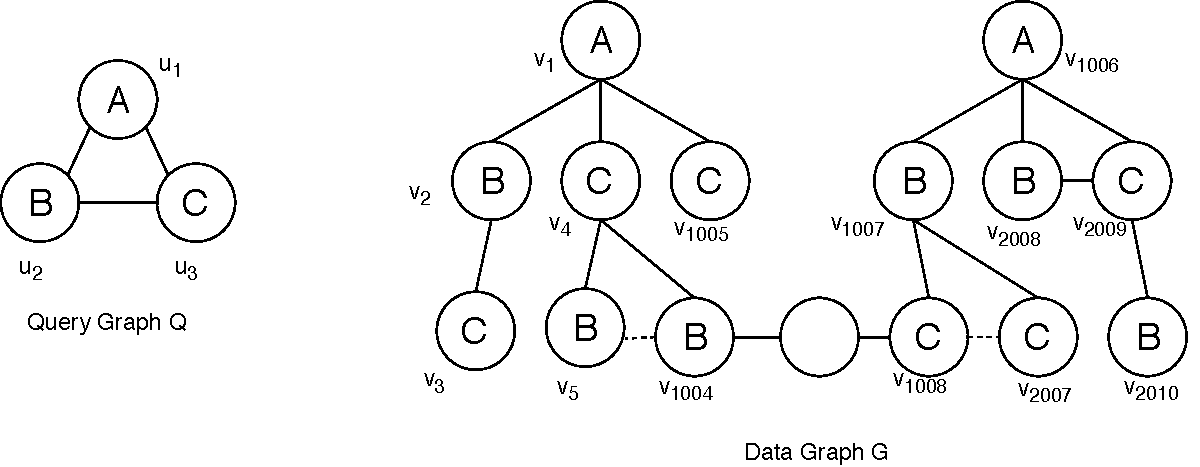
\includegraphics[width=\columnwidth]{images/graph.pdf}
\caption[Subgraph Isomorphism]{A query graph $q$ and a data graph $g$} % The text in the square bracket is the caption for the list of figures while the text in the curly brackets is the figure caption
\label{fig:gallery} 
\end{figure}

For the above query graph, the data subgraph {$v_{1006}, v_{2008}, v_{2009}$} is isomorphic to the query graph and hence is a match. There is no other match for the given query graph in the data graph.

\section{Data Representation}

In the implementation, graphs are represented as compressed sparse rows(CSR). The CSR representation of a matrix consists of several one dimensional arrays. The number of arrays depends upon the information carried by the matrix. For example, consider the adjacency matrix of a labelled graph with 9 vertices as shown in the figure below. For this graph, the CSR representation will contain 3 vectors (1-d arrays), namely IA, JA and LA, which are defined as:

IA is an array of size rows(M) + 1 which is recursively defined as:
\begin{itemize}
    \item $IA[0] = 0$
    \item $IA[i]$ = $IA[i - 1]$ + number of non zero entries in $i - 1^{th}$ row of M
\end{itemize}

JA is an array of size equal to value last element of IA i.e. the number of edges in the graph. The entries of JA are the column numbers of all the non zero entries of from left to right row-wise.

LA is an array of size rows(M). It contains the labels of all the nodes in order. For the graph in figure 1.2, the matrix M and CSR representation are given.

\begin{figure}[h]
\centering 
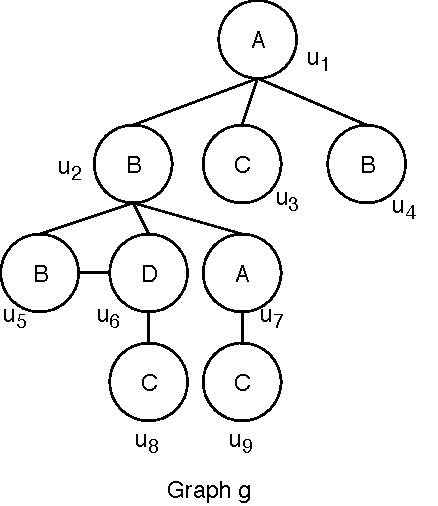
\includegraphics[scale = 0.8]{images/csr.pdf}
\caption[Graph representation]{Graph representation : graph $g$} % The text in the square bracket is the caption for the list of figures while the text in the curly brackets is the figure caption
\label{fig:gallery} 
\end{figure}

\[
    M =
    \begin{bmatrix}
        0 & 1 & 1 & 1 & 0 & 0 & 0 & 0 & 0\\
        1 & 0 & 0 & 0 & 1 & 1 & 1 & 0 & 0\\
        1 & 0 & 0 & 0 & 0 & 0 & 0 & 0 & 0\\
        1 & 0 & 0 & 0 & 0 & 0 & 0 & 0 & 0\\
        0 & 1 & 0 & 0 & 0 & 1 & 0 & 0 & 0\\
        0 & 1 & 0 & 0 & 1 & 0 & 0 & 1 & 0\\
        0 & 1 & 0 & 0 & 0 & 0 & 0 & 0 & 1\\
        0 & 0 & 0 & 0 & 0 & 1 & 0 & 0 & 0\\
        0 & 0 & 0 & 0 & 0 & 0 & 1 & 0 & 0\\
    \end{bmatrix}
\]
\\
\[
    IA = 
    \begin{bmatrix}
        0 & 3 & 7 & 8 & 9 & 11 & 14 & 16 & 17 & 18
    \end{bmatrix}
\] 
\[
    JA =
    \begin{bmatrix}
        1 & 2 & 3 & 0 & 4 & 5 & 6 & 0 & 0 & \dots
    \end{bmatrix}
\]
\[
    LA =
    \begin{bmatrix}
        A & B & C & B & B & D & A & C & C
    \end{bmatrix}
\]


\section{CUDA Architecture}

Figure 1.3 gives an overview of modern day GPU architecture. \cite{book} has been referred for CUDA related concepts. CUDA enabled GPU is made up of number of highly threaded streaming microprocessors. In the figure, there are 2 streaming multiprocessors in each building block. Each of these streaming microprocessors is itself made up of streaming processors (6 SPs per SM in figure 2). These steaming processors share control logic and instruction cache.The global memory is made of DRAM and has very high bandwidth. Although the GPU global memory has higher latency as compared to the CPU RAM, highly parallel applications can compensate for the latency as it has higher bandwidth resulting in superior execution time.

\begin{figure}[h]
\centering 
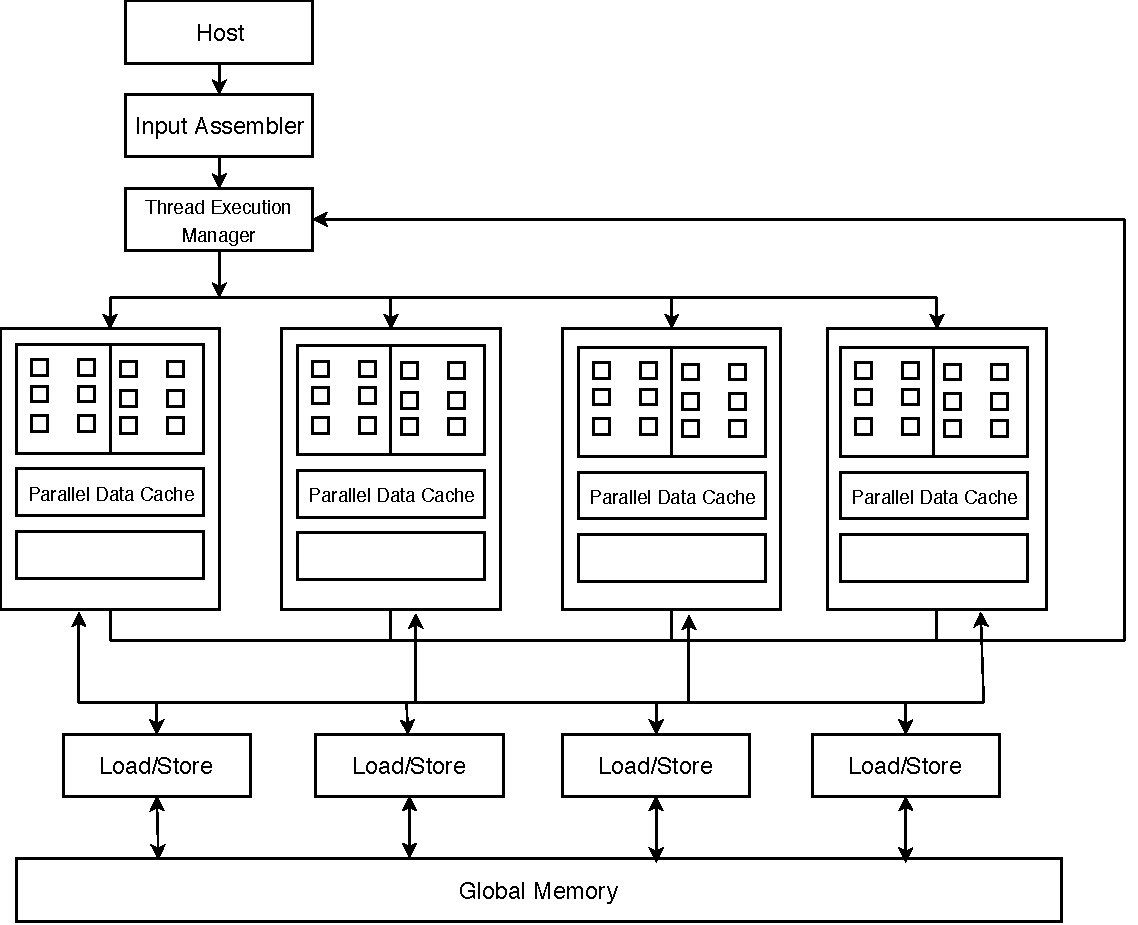
\includegraphics[width=\columnwidth]{images/gpu.pdf} 
\caption[CUDA architecture]{CUDA enabled GPU architecture} % The text in the square bracket is the caption for the list of figures while the text in the curly brackets is the figure caption
\label{fig:gallery} 
\end{figure}

\section{Organization of the Thesis}
Chapter \ref{chap:lit} discusses the previous works in this area and related concepts. In Chapter 3, the parallel implementation is discussed with example. Chapter 4 discusses the comparative study of performances of the sequential and the parallel implementations. The datasets on with the study is done are also explained in this section. Chapter 5 concludes the work with analysis and proposes future work and optimizations that can be done to improve the speedup.